\documentclass[11pt]{article}

\usepackage[a4paper,margin=0.92in]{geometry}
\usepackage[T1]{fontenc}
\usepackage[utf8]{inputenc}
\usepackage{lmodern}
\usepackage{microtype}
\usepackage{amsmath,amssymb,amsthm,mathtools}
\usepackage{booktabs,array}
\usepackage{graphicx}
\usepackage{enumitem}
\usepackage{xcolor}
\usepackage[hidelinks]{hyperref}

\emergencystretch=2em

\graphicspath{{../figures/}}

\hypersetup{
  pdftitle={Pandrosion Relativity},
  pdfauthor={Ivan Besevic},
  pdfsubject={Finite-slope Pandrosion formulation of relativistic geodesic motion},
  pdfkeywords={Pandrosion, relativity, geodesics, Lorentzian geometry, causal probes, dynamic atlases}
}

\newtheorem{definition}{Definition}[section]
\newtheorem{assumption}[definition]{Assumption}
\newtheorem{lemma}[definition]{Lemma}
\newtheorem{theorem}[definition]{Theorem}
\newtheorem{proposition}[definition]{Proposition}
\newtheorem{corollary}[definition]{Corollary}
\newtheorem{conjecture}[definition]{Conjecture}
\newtheorem{remark}[definition]{Remark}

\newcommand{\R}{\mathbb R}
\newcommand{\M}{\mathcal M}
\newcommand{\A}{\mathcal A}
\newcommand{\Cset}{\mathcal C}
\newcommand{\D}{\mathcal D}
\newcommand{\G}{\mathcal G}
\newcommand{\J}{\mathcal J}
\newcommand{\K}{\mathcal K}
\newcommand{\N}{\mathcal N}
\newcommand{\Pset}{\mathcal P}
\newcommand{\T}{\mathcal T}
\newcommand{\U}{\mathcal U}
\newcommand{\V}{\mathcal V}
\newcommand{\dd}{\,\mathrm d}
\newcommand{\Oterm}{\mathcal O}
\newcommand{\norm}[1]{\left\lVert #1\right\rVert}
\DeclareMathOperator*{\argmax}{arg\,max}
\DeclareMathOperator*{\argmin}{arg\,min}
\DeclareMathOperator{\Exp}{Exp}
\DeclareMathOperator{\dist}{dist}
\DeclareMathOperator{\Ric}{Ric}
\DeclareMathOperator{\tr}{tr}

\title{Pandrosion Relativity\\[3pt]
\large Finite-slope causal probes, dynamic atlases, and geodesic physical motion}
\author{Ivan Besevic\\Independent Mathematical Research}
\date{May 2026}

\begin{document}
\maketitle

\begin{abstract}
This paper develops a ``Pandrosion relativity'' formulation.  It does not
replace special or general relativity.  Instead, it rewrites the relativistic
motion law as a finite-slope Pandrosion probe calculus: admissible probes must
stay inside the future light cone, massive-particle paths are selected by a
discrete proper-time score, and dynamic atlases remove coordinate defects in
the same spirit as Thales scaling and Riemann-chart inversion in monomial
Pandrosion.

Let \((\M,g)\) be a time-oriented Lorentzian manifold.  A Pandrosion worldline
is a causal graph path
\[
        \Gamma=(p_0,p_1,\ldots,p_N),
        \qquad p_{k+1}\in\Cset_h^+(p_k),
\]
with score
\[
        \begin{aligned}
        \J_h(\Gamma)
        &=
        \sum_{k=0}^{N-1}\tau_h(p_k,p_{k+1})
        -
        \lambda_h\sum_k\A_h(p_{k-1},p_k,p_{k+1})
\\
        &\quad
        -
        \mu_h\sum_k\K_h(p_k,p_{k+1})
        -
        \nu_h\sum_k\Theta_h(p_k,p_{k+1}).
        \end{aligned}
\]
Here \(\tau_h\) is the finite-segment proper time, \(\A_h\) penalizes
finite-slope acceleration, \(\K_h\) penalizes curvature or tidal stiffness, and
\(\Theta_h\) penalizes ill-conditioned charts.  The main theorem states that,
on a compact globally hyperbolic domain and under causal graph consistency,
maximizers of \(\J_h\) converge to proper-time maximizing causal geodesics as
\(h\to0\), when the penalty weights vanish at a consistent rate.  A second
result shows that the dynamic-atlas formulation is chart invariant in the
continuum limit.  Finally, the weak-field slow-motion expansion recovers
Newton's law, while a finite-holonomy conjecture gives the natural Pandrosion
route toward Einstein's field equation.
\end{abstract}

\paragraph{One-sentence summary.}
Pandrosion relativity is a finite-probe version of relativistic geodesic
motion: replace derivatives by causal finite slopes, replace one coordinate
system by a dynamic atlas, and recover standard relativity in the continuum
limit.

\paragraph{Status.}
The graph-convergence and chart-covariance statements are mathematical
approximation theorems under explicit consistency hypotheses.  The finite
curvature-to-field-equation step is stated as a research conjecture, not as a
new proof of general relativity.

\tableofcontents

\section{Purpose of the paper}

The previous Pandrosion papers built three ideas that naturally touch
relativity:
\begin{enumerate}[label=(\roman*)]
\item Paper 000 showed that a useful computation may require a chart choice,
a homothety, and sometimes a reciprocal Riemann chart.
\item Papers 011--013 treated probes as geodesic objects selected by a
stability metric.
\item Paper 019 proved that dense finite probe graphs can converge to
continuous geodesic actions.
\end{enumerate}
Relativity is also a geometric theory.  The free motion of a massive particle
is not defined by a preferred coordinate acceleration.  It is defined by a
causal path that extremizes proper time and is independent of the chart used to
describe it.

This makes a clean Pandrosion translation possible.  The derivative of a
worldline is replaced by finite causal segments.  The Christoffel-symbol
geodesic equation is replaced by a finite-slope transport condition.  Bad
coordinates are treated as chart defects, not as physical singularities.  The
resulting method is not a new physical law; it is a finite-probe language for
the existing relativistic law.

\begin{figure}[htbp]
\centering
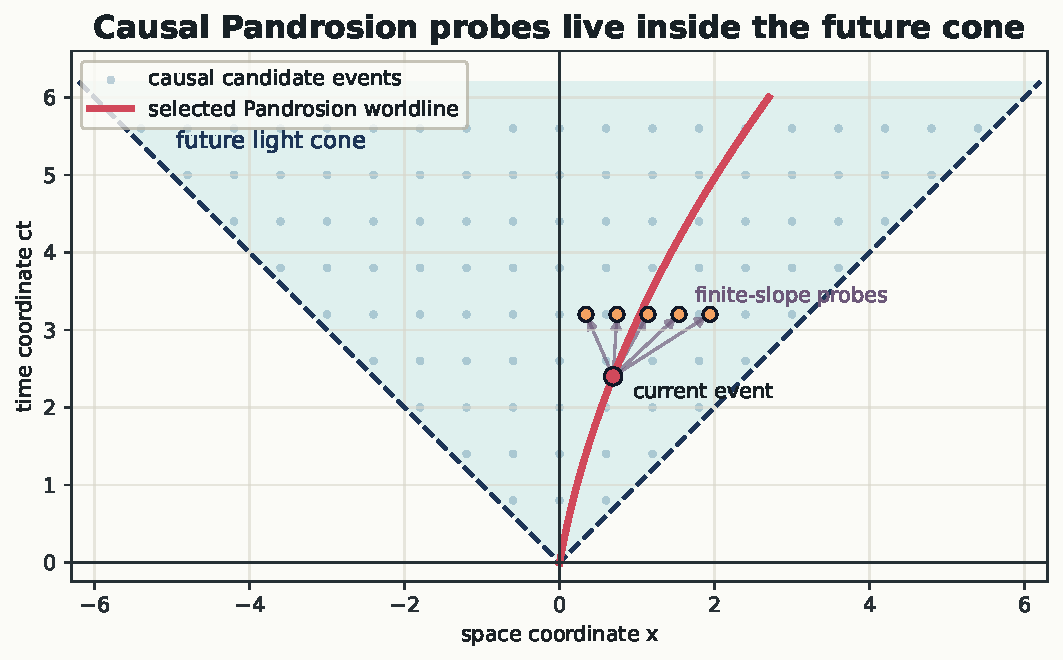
\includegraphics[width=0.82\linewidth]{027_causal_probe_lattice.pdf}
\caption{Causal Pandrosion probe geometry.  The candidate endpoint set is not
Euclidean; it is restricted by the future light cone.  A worldline is selected
from finite causal probes by a proper-time score plus finite-slope and atlas
penalties.}
\label{fig:causal-probes}
\end{figure}

\section{Relativistic Pandrosion state}

Let \((\M,g)\) be a smooth time-oriented Lorentzian manifold of dimension
\(d+1\), with signature \((-+\cdots+)\).  We use units \(c=1\) until the
Newtonian limit section.  A future-directed tangent vector \(v\) is timelike
when
\[
        g_p(v,v)<0.
\]
The proper time of a timelike \(C^1\) curve \(\gamma\) is
\[
        \T(\gamma)
        =
        \int\sqrt{-g_{\gamma(t)}(\dot\gamma(t),\dot\gamma(t))}\,\dd t.
\]

\begin{definition}[Pandrosion relativistic state]
A relativistic Pandrosion state is
\[
        \mathfrak s=(p,i,e,\rho),
\]
where \(p\in\M\) is the current event, \(i\) is the active chart or tetrad
index, \(e\) is a local future timelike frame vector, and \(\rho>0\) is the
current probe scale.
\end{definition}

The scale \(\rho\) is the relativistic analog of Thales normalization.  It
keeps probe segments inside a local region where the metric, chart transition,
and finite-slope estimates are stable.  The chart index \(i\) is the analog of
the direct or reciprocal Riemann chart in Paper 000: it is not physics, but it
controls numerical stability.

\begin{definition}[Causal probe set]
Let \(X_h\subset\M\) be a finite event set with mesh size \(h\).  The future
causal Pandrosion probe set at \(p\in X_h\) is
\[
        \Cset_h^+(p)
        =
        \{q\in X_h:\ q\in J^+(p),\ h_-\le \tau_h(p,q)\le h_+\},
\]
where \(J^+(p)\) is the causal future of \(p\), \(0<h_-\le h_+\), and
\(\tau_h(p,q)\) is a local finite-segment proper-time estimator.
\end{definition}

In a chart \(\phi_i\), write \(\Delta x^\alpha=x^\alpha(q)-x^\alpha(p)\).
For sufficiently small segments one may use
\[
        \tau_{h,i}(p,q)
        =
        \sqrt{\max\{0,-g^{(i)}_{\alpha\beta}(p)\Delta x^\alpha\Delta x^\beta\}}.
\]
Higher-order quadrature may replace this first-order estimator.  The important
point is that the endpoint is admissible only if the finite segment is
future-causal.

\section{Finite-slope proper-time score}

A discrete Pandrosion worldline is a graph path
\[
        \Gamma=(p_0,p_1,\ldots,p_N),
        \qquad p_{k+1}\in\Cset_h^+(p_k).
\]
The raw discrete proper time is
\[
        \T_h(\Gamma)
        =
        \sum_{k=0}^{N-1}\tau_h(p_k,p_{k+1}).
\]
For a free massive particle, the continuum law says that the physical path is
a proper-time extremal.  In a convex normal neighborhood this is a local
maximum of proper time among nearby timelike curves with fixed endpoints.
Pandrosion therefore uses a maximizing score, not a descent score:
\[
        \J_h(\Gamma)
        =
        \T_h(\Gamma)-\Pset_h(\Gamma).
\]
The penalty \(\Pset_h\) contains the terms that make finite probes stable.

\begin{definition}[Pandrosion relativistic score]
For \(\Gamma=(p_0,\ldots,p_N)\), set
\[
\begin{aligned}
        \J_h(\Gamma)
        &=
        \sum_{k=0}^{N-1}\tau_h(p_k,p_{k+1})
        -
        \lambda_h\sum_{k=1}^{N-1}
        \A_h(p_{k-1},p_k,p_{k+1})
\\
        &\quad
        -
        \mu_h\sum_{k=0}^{N-1}
        \K_h(p_k,p_{k+1})
        -
        \nu_h\sum_{k=0}^{N-1}
        \Theta_h(p_k,p_{k+1}).
\end{aligned}
\]
Here \(\A_h\) is a finite-slope acceleration penalty, \(\K_h\) is a curvature
or tidal-stiffness penalty, and \(\Theta_h\) is a chart-conditioning penalty.
\end{definition}

The penalty terms are not external forces.  They are numerical stabilizers.
For a continuum convergence theorem, their weights should vanish as
\(h\to0\).  For a practical engine, they prevent a finite graph from choosing
segments that are formally causal but unstable because of a poor chart, a
large tidal gradient, or a noisy finite-slope estimate.

\subsection{Finite-slope connection}

Let \(g_{\alpha\beta}\) be sampled on a local event lattice.  A finite
difference \(D^h_\mu g_{\alpha\beta}(p)\) gives the finite-slope Christoffel
symbol
\[
        \Gamma_{h,\alpha\beta}^{\mu}(p)
        =
        \frac12 g_h^{\mu\nu}(p)
        \left(
        D^h_\alpha g_{\beta\nu}(p)
        +
        D^h_\beta g_{\alpha\nu}(p)
        -
        D^h_\nu g_{\alpha\beta}(p)
        \right).
\]
For a graph path, define segment velocities
\[
        V_k^\mu
        =
        \frac{x^\mu(p_{k+1})-x^\mu(p_k)}{\Delta t_k}.
\]
A finite-slope geodesic defect is then
\[
        E^\mu_{h,k}
        =
        \frac{V_{k+1}^\mu-V_k^\mu}{\Delta t_k}
        +
        \Gamma_{h,\alpha\beta}^{\mu}(p_k)V_k^\alpha V_k^\beta.
\]
The acceleration penalty may be chosen as
\[
        \A_h(p_{k-1},p_k,p_{k+1})
        =
        \sum_{\mu}|E^\mu_{h,k}|^2\,\Delta t_k.
\]
Thus the usual differential equation
\[
        \ddot x^\mu+\Gamma^\mu_{\alpha\beta}\dot x^\alpha\dot x^\beta=0
\]
is recovered as the zero-defect limit of finite-slope probes.

\section{Main convergence theorem}

The next theorem is the relativistic analog of the graph-action theorem in
Paper 019.  The sign changes because timelike geodesics maximize proper time
locally, while the Riemannian stability actions in Paper 019 minimized length.

\begin{assumption}[Causal graph consistency]\label{ass:causalgraph}
Let \(\D\subset\M\) be a compact causally convex subset of a globally
hyperbolic spacetime, and let \(p_-,p_+\in\D\) be timelike related.  A family
of finite event graphs \(X_h\subset\D\) is causally consistent if:
\begin{enumerate}[label=(\roman*)]
\item the mesh of \(X_h\) in \(\D\) tends to zero;
\item graph edges are future-causal and have maximum coordinate size
\(\Oterm(h)\);
\item every smooth future-timelike curve in \(\D\) can be uniformly sampled by
future-causal graph paths;
\item the segment estimator satisfies
\[
        \tau_h(a,b)
        =
        \tau_{\mathrm{geo}}(a,b)+\Oterm(h^3)
\]
uniformly for small timelike segments, where \(\tau_{\mathrm{geo}}(a,b)\) is
the geodesic proper time between nearby events.
\end{enumerate}
\end{assumption}

\begin{assumption}[Vanishing stabilizers]\label{ass:stabilizers}
The penalties in \(\J_h\) are nonnegative and satisfy
\[
        \sup_{\Gamma\in\G_h}
        \left[
        \lambda_h\sum \A_h
        +
        \mu_h\sum \K_h
        +
        \nu_h\sum \Theta_h
        \right]
        \longrightarrow 0
\]
on every uniformly bounded family of consistent timelike graph paths
\(\G_h\).
\end{assumption}

\begin{theorem}[Pandrosion causal graph convergence]\label{thm:causal-convergence}
Assume causal graph consistency and vanishing stabilizers.  Let
\(\Gamma_h\) maximize \(\J_h\) among future-causal graph paths from nodes
converging to \(p_-\) to nodes converging to \(p_+\).  If the polygonal
interpolants of \(\Gamma_h\) have a uniformly convergent subsequence, then
every subsequential limit \(\gamma\) is a proper-time maximizing future-causal
curve from \(p_-\) to \(p_+\).  On a smooth timelike interior where the
maximizer is regular, \(\gamma\) is a timelike geodesic.  If the maximizing
geodesic is unique, the full family \(\Gamma_h\) converges to it.
\end{theorem}

\begin{proof}
Let
\[
        \T_*(p_-,p_+)
        =
        \sup_{\eta}\T(\eta),
\]
where the supremum is over future-causal curves from \(p_-\) to \(p_+\) in
\(\D\).  By global hyperbolicity and compactness of \(\D\), maximizing causal
curves exist.

For the lower bound, take a smooth timelike curve \(\eta\) whose proper time is
within \(\varepsilon\) of \(\T_*\).  Causal graph consistency supplies graph
paths \(\Gamma_h^\eta\) converging uniformly to \(\eta\).  The segment
estimator is consistent, so
\[
        \lim_{h\to0}\T_h(\Gamma_h^\eta)=\T(\eta).
\]
The stabilizers vanish on these paths, hence
\[
        \liminf_{h\to0}\sup_{\Gamma}\J_h(\Gamma)
        \ge \T(\eta)
        \ge \T_*-\varepsilon.
\]
Letting \(\varepsilon\to0\) gives the recovery inequality.

For the upper bound, let \(\Gamma_{h_j}\) be a maximizing subsequence whose
interpolants converge uniformly to \(\gamma\).  Lorentzian length is upper
semicontinuous for uniformly convergent causal curves in a globally hyperbolic
domain, and the local segment estimator differs from geodesic proper time by
an error summing to \(o(1)\).  Since the penalties are nonnegative,
\[
        \limsup_{j\to\infty}\J_{h_j}(\Gamma_{h_j})
        \le
        \limsup_{j\to\infty}\T_{h_j}(\Gamma_{h_j})
        \le
        \T(\gamma)
        \le
        \T_*.
\]
Together with the lower bound, \(\T(\gamma)=\T_*\), so \(\gamma\) maximizes
proper time.  A regular timelike proper-time extremal satisfies the geodesic
equation.  Uniqueness removes the need to pass to subsequences.
\end{proof}

\begin{corollary}[Finite-slope geodesic equation]\label{cor:finite-slope}
Under the hypotheses of Theorem~\ref{thm:causal-convergence}, if the finite
metric differences \(D^h g\) converge uniformly to \(\partial g\) on the
limiting tube, then the finite-slope defects \(E^\mu_{h,k}\) converge weakly to
zero along any regular interior segment of the limiting worldline.
\end{corollary}

\begin{proof}
The graph maximizers converge to a regular timelike geodesic.  Uniform
convergence of \(D^h g\) to \(\partial g\) gives convergence of
\(\Gamma_h\) to the Levi-Civita symbols.  The discrete Euler condition for
nearby probe variations is therefore the finite-difference form of the
geodesic Euler--Lagrange equation, with consistency error tending to zero.
\end{proof}

\section{Dynamic atlas and horizon-safe charting}

Coordinate singularities are a central reason to use an atlas rather than a
single chart.  The Schwarzschild radial coordinate is a standard example: the
coordinate expression has a singularity at \(r=2M\), but the horizon is not a
curvature singularity.  A Pandrosion engine should treat this as a chart
conditioning problem.

\begin{figure}[htbp]
\centering
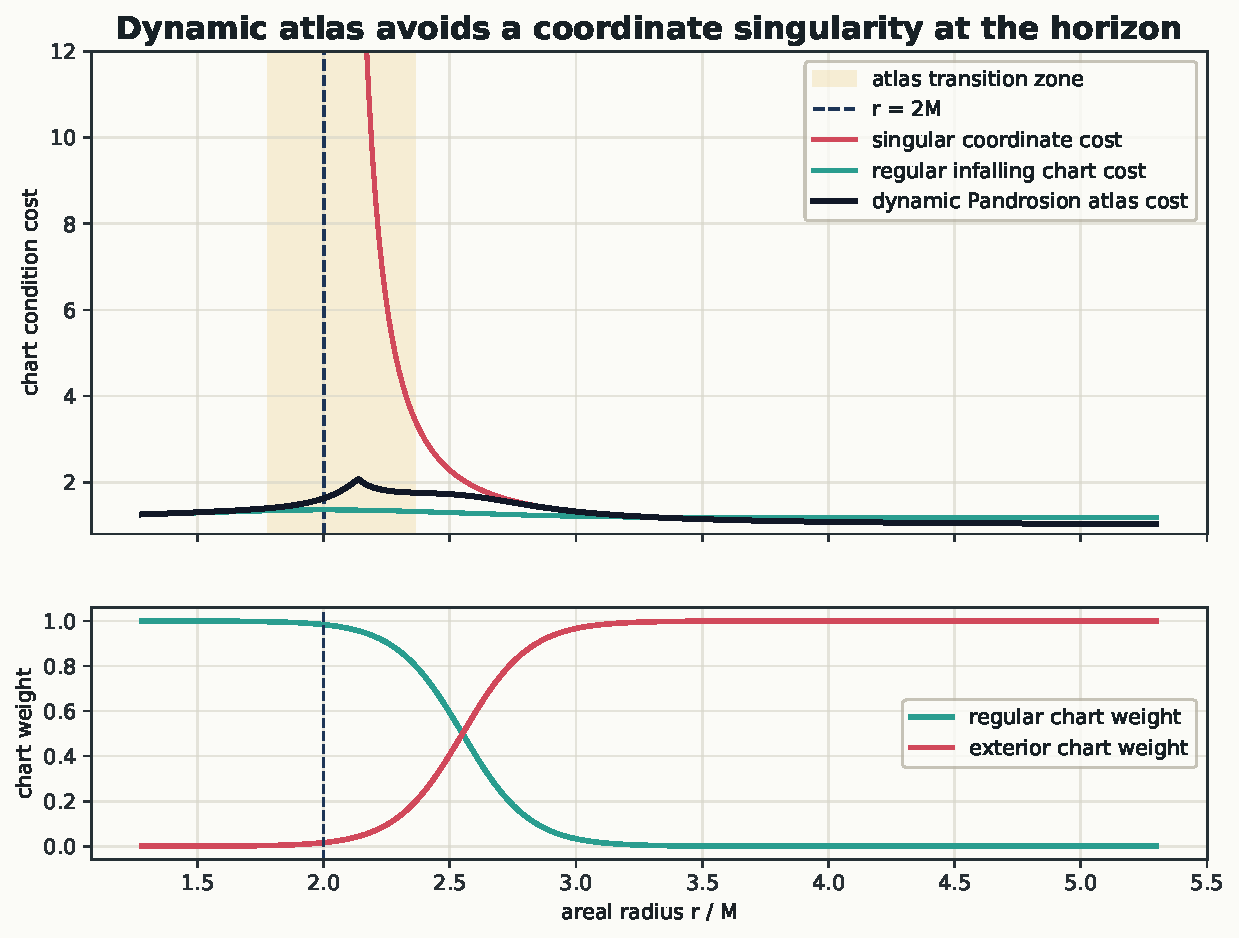
\includegraphics[width=0.92\linewidth]{027_dynamic_atlas_horizon.pdf}
\caption{Dynamic chart selection near a horizon.  A coordinate chart may become
ill-conditioned even when the spacetime geometry is regular.  The Pandrosion
atlas switches to a regular infalling chart near the bad coordinate region and
returns to the exterior chart away from it.}
\label{fig:dynamic-horizon}
\end{figure}

Let \(\{(U_i,\phi_i)\}_{i\in I}\) be a smooth atlas on \(\D\).  A charted
worldline stores
\[
        (p_0,i_0),(p_1,i_1),\ldots,(p_N,i_N).
\]
For an edge \((p_k,p_{k+1})\), the local segment time is evaluated in chart
\(i_k\), while the transition \(i_k\to i_{k+1}\) is charged a small atlas cost
\[
        \Theta_h(p_k,p_{k+1},i_k,i_{k+1})
        =
        \theta_i(p_k)+\theta_j(p_{k+1})
        +
        \sigma_h\,\norm{D\phi_j\circ D\phi_i^{-1}}.
\]
Here \(\theta_i\) measures chart conditioning.  It is allowed to grow near a
coordinate defect, forcing the optimizer to select a better chart.

\begin{proposition}[Local chart covariance]\label{prop:chart-covariance}
Let two charts \(i,j\) overlap on a compact region and have bounded
derivatives through order three.  If a segment has size \(h\), then the
first-order finite-segment proper-time estimators computed in the two charts
satisfy
\[
        \tau_{h,i}(p,q)-\tau_{h,j}(p,q)=\Oterm(h^3).
\]
Consequently, along a path with \(\Oterm(h^{-1})\) segments and bounded total
time, the total chart discrepancy is \(\Oterm(h^2)\).
\end{proposition}

\begin{proof}
The exact quadratic expression
\(-g_p(v,v)\) is tensorial.  The only difference between chart estimators comes
from representing the finite displacement \(q-p\) by first-order chart
increments instead of the exact exponential displacement.  Taylor expansion of
the chart transition map gives an error of order \(h^3\) in the segment proper
time on compact overlaps.  Summing over \(\Oterm(h^{-1})\) segments gives
\(\Oterm(h^2)\).
\end{proof}

\begin{theorem}[Dynamic-atlas invariance]\label{thm:atlas}
Assume the hypotheses of Theorem~\ref{thm:causal-convergence} and let the
atlas transition weights vanish while still excluding charts whose condition
cost diverges.  Then the limiting Pandrosion worldline is independent of the
chosen smooth atlas.  Different atlases may choose different finite graph
paths, but every convergent maximizing family has the same continuum
proper-time maximizer when that maximizer is unique.
\end{theorem}

\begin{proof}
On every compact overlap the segment-time discrepancy between smooth charts is
summable to \(o(1)\) by the chart-covariance proposition.  Divergent chart
costs only remove ill-conditioned coordinate descriptions; they do not remove
the underlying event from the manifold if another regular chart covers it.
Therefore all admissible smooth atlases produce the same limiting proper-time
functional.  The causal graph convergence theorem then applies.
\end{proof}

\section{Relation to Thales scaling and Riemann inversion}

The terminology in Paper 000 can be translated almost literally.

\begin{table}[htbp]
\centering
\renewcommand{\arraystretch}{1.22}
\begin{tabular}{>{\raggedright\arraybackslash}p{0.28\linewidth}>{\raggedright\arraybackslash}p{0.31\linewidth}>{\raggedright\arraybackslash}p{0.31\linewidth}}
\toprule
Monomial Pandrosion & Relativistic Pandrosion & Meaning \\
\midrule
Thales homothety & local inertial normalization & choose a scale where finite probes see a nearly flat metric \\
Riemann inversion & switch to a nonsingular spacetime chart & avoid a coordinate defect without changing the event \\
finite slope & causal segment difference & replace derivatives of the worldline by finite causal probes \\
equal-value pole barrier & caustic, chart, or curvature barrier & keep probes away from regions where finite information collapses \\
geodesic probe score & proper-time graph score & choose paths by an invariant action rather than by raw coordinates \\
\bottomrule
\end{tabular}
\caption{Dictionary from the earlier Pandrosion papers to the relativistic
version.  The physical invariant is not the chart; it is the proper-time
functional and the causal structure.}
\label{tab:dictionary}
\end{table}

This is the clean answer to the question ``can Pandrosion replace Newton?''.
Newton's law is not replaced at the fundamental level; it appears as the
weak-field, slow-motion limit of relativistic proper-time maximization.
Pandrosion supplies the finite-probe mechanism that approximates that
geometric law.

\section{Newtonian limit}

Restore \(c\).  In a weak static field with Newtonian potential \(\Phi\), use
the standard first post-Newtonian metric model
\[
        \dd s^2
        =
        -
        \left(1+\frac{2\Phi}{c^2}\right)c^2\dd t^2
        +
        \left(1-\frac{2\Phi}{c^2}\right)\norm{\dd x}^2
        +
        \Oterm(c^{-4}).
\]
For a slow path \(x(t)\), \(\norm{\dot x}\ll c\), the proper time satisfies
\[
\begin{aligned}
        \dd\tau
        &=
        \frac{1}{c}\sqrt{-\dd s^2}
\\
        &=
        \left[
        1+\frac{\Phi(x)}{c^2}
        -
        \frac{\norm{\dot x}^2}{2c^2}
        \right]\dd t
        +
        \Oterm(c^{-4})+\Oterm(\norm{\dot x}^4/c^4).
\end{aligned}
\]
Thus maximizing \(\int\dd\tau\) is equivalent, up to an additive constant and a
positive factor, to minimizing
\[
        \int
        \left(
        \frac12\norm{\dot x}^2-\Phi(x)
        \right)\dd t.
\]
The Euler--Lagrange equation is
\[
        \ddot x=-\nabla\Phi(x).
\]

\begin{theorem}[Newtonian shadow of Pandrosion relativity]
Let the hypotheses of Theorem~\ref{thm:causal-convergence} hold in a weak
static field, and assume all selected graph paths remain in the slow-motion
regime.  Then the spatial projections of maximizing Pandrosion worldlines
converge, after the weak-field expansion, to solutions of Newton's equation
\[
        \ddot x=-\nabla\Phi(x)
\]
with the same endpoint data.
\end{theorem}

\begin{proof}
Theorem~\ref{thm:causal-convergence} gives convergence to a proper-time
maximizing timelike geodesic.  The weak-field expansion above converts
proper-time maximization into the classical action principle with Lagrangian
\(\frac12\norm{\dot x}^2-\Phi(x)\).  Its Euler--Lagrange equation is Newton's
law.
\end{proof}

\section{Finite holonomy and curvature}

Geodesic motion uses the metric as input.  General relativity also determines
the metric through curvature.  A Pandrosion route to the field equation should
therefore begin with finite curvature measurements, not with symbolic
derivatives.

\begin{figure}[htbp]
\centering
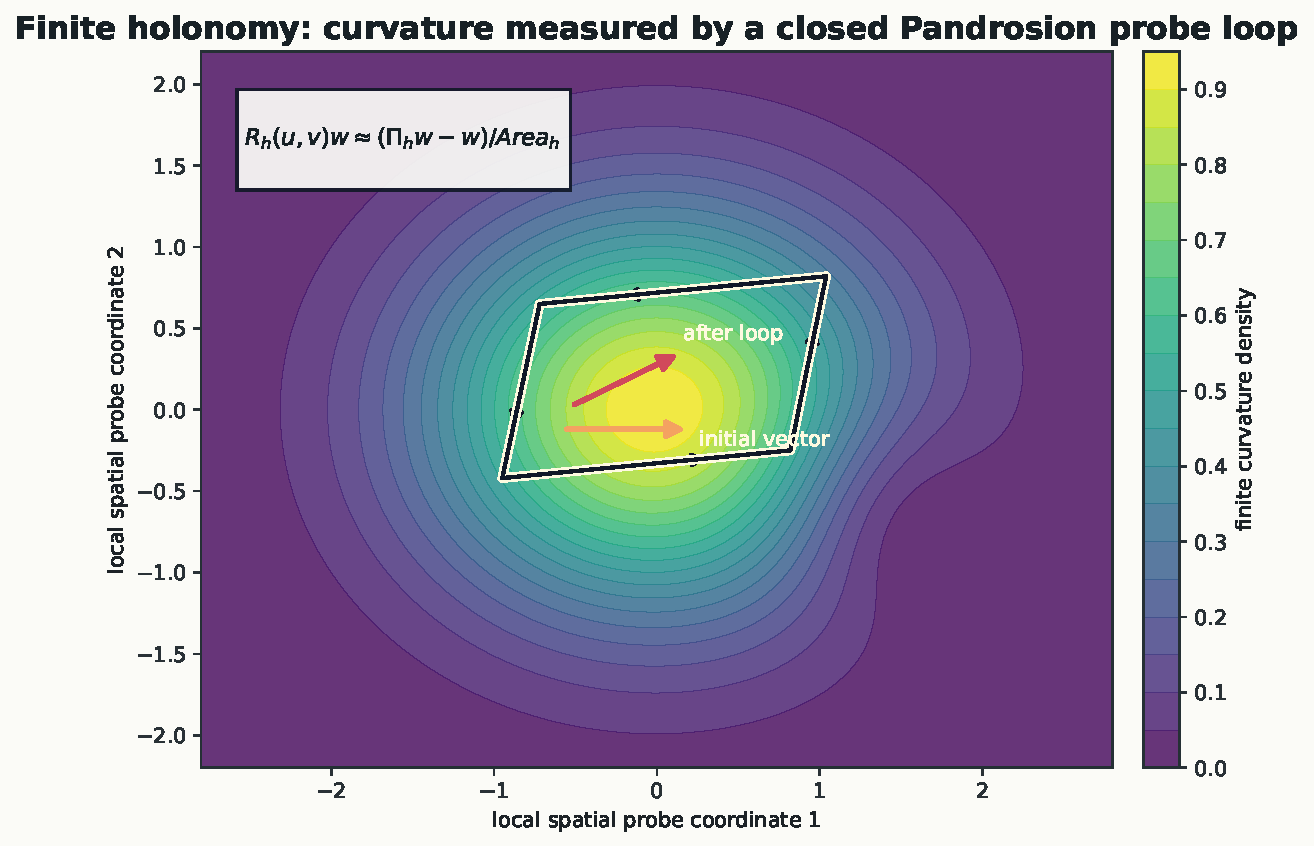
\includegraphics[width=0.86\linewidth]{027_finite_holonomy_curvature.pdf}
\caption{Finite holonomy curvature.  Parallel transport around a small closed
probe loop returns a vector with a finite rotation.  Dividing the defect by the
loop area gives a finite-slope curvature estimator.}
\label{fig:holonomy}
\end{figure}

Let \(\Pi_{h,\square}\) be finite parallel transport around a small loop
\(\square_h(u,v)\) spanned by two probe directions \(u,v\).  Define
\[
        R_h(u,v)w
        =
        \frac{\Pi_{h,\square}w-w}{\operatorname{Area}_h(u,v)}.
\]
If the transport rule is consistent with the Levi-Civita connection, then this
is the natural Pandrosion estimator for the Riemann curvature tensor.

\begin{conjecture}[Finite holonomy convergence]
On compact regions where the metric is \(C^3\) and the finite transport rule is
second-order consistent with Levi-Civita transport,
\[
        R_h(u,v)w
        \longrightarrow
        R(u,v)w
\]
uniformly for bounded probe directions as \(h\to0\).
\end{conjecture}

Assuming this convergence, one can form finite Ricci and scalar curvature
estimators by contraction:
\[
        \Ric_h(u,v)=\tr[w\mapsto R_h(w,u)v],
        \qquad
        S_h=\tr_g\Ric_h,
\]
and then the finite Einstein tensor
\[
        G_h=\Ric_h-\frac12 S_h g_h.
\]

\begin{conjecture}[Pandrosion field balance]
A finite-probe formulation of the Einstein equation should take the form
\[
        G_h+\Lambda g_h
        =
        \frac{8\pi G}{c^4}T_h+o(1),
\]
where \(T_h\) is a finite-volume stress-energy estimator.  If the holonomy,
contraction, and stress-energy estimators are consistent, the limit is the
classical Einstein equation
\[
        G+\Lambda g
        =
        \frac{8\pi G}{c^4}T.
\]
\end{conjecture}

This conjecture is deliberately conservative.  It does not assert a new
physical equation.  It states that the Pandrosion way to make the equation
finite is through holonomy loops, atlas conditioning, and causal probes.

\section{Practical algorithm}

A numerical Pandrosion-relativity engine can be written as a finite pipeline.

\begin{enumerate}[label=\textbf{Step \arabic*.},leftmargin=*]
\item Build a local event cloud \(X_h\) around the current event \(p_k\).
\item Remove endpoints outside the future cone, producing \(\Cset_h^+(p_k)\).
\item For each candidate, compute finite proper time, chart condition, tidal
stiffness, and finite-slope acceleration defect.
\item Select the next event or a short graph path by maximizing \(\J_h\).
\item Update the active chart by minimizing the atlas condition cost.
\item Repeat until the target hypersurface or endpoint neighborhood is reached.
\end{enumerate}

In flat Minkowski space, this engine selects straight timelike lines between
fixed endpoints.  In a curved spacetime, it selects discrete approximations to
timelike geodesics.  Near a coordinate singularity, it should switch charts
rather than misreading the coordinate blow-up as a physical force.

\section{What is new here}

The formulas of relativity themselves are classical.  The new Pandrosion
contribution is the organization:
\begin{enumerate}[label=(\roman*)]
\item a causal finite-slope probe set replaces infinitesimal tangent vectors;
\item a maximizing graph score replaces the differential geodesic equation;
\item dynamic atlas conditioning replaces dependence on a single coordinate
system;
\item Thales-style scale normalization becomes local inertial normalization;
\item finite holonomy provides the curvature estimator needed for a future
field-equation discretization.
\end{enumerate}
This is enough to make a genuine research program: prove sharper convergence
rates, test chart-selection rules near horizons and caustics, and compare
finite-holonomy field balances with standard Regge calculus or finite-volume
relativity.

\section{Conclusion}

Pandrosion relativity is best read as a finite geometric calculus for the
standard relativistic principle of motion.  It respects the causal cone,
maximizes proper time for massive free particles, uses dynamic atlases to avoid
coordinate artifacts, and converges to timelike geodesics under graph
consistency.  In the weak-field slow-motion limit it gives Newton's law.  The
next frontier is not to claim a replacement for Einstein's equation, but to
build a finite-holonomy Pandrosion version of curvature and stress-energy that
converges to it.

\begin{thebibliography}{9}
\bibitem{einstein1915}
A. Einstein, \emph{Die Feldgleichungen der Gravitation}, Sitzungsberichte der
Preussischen Akademie der Wissenschaften, 1915.

\bibitem{wald}
R. M. Wald, \emph{General Relativity}, University of Chicago Press, 1984.

\bibitem{oneill}
B. O'Neill, \emph{Semi-Riemannian Geometry}, Academic Press, 1983.

\bibitem{regge}
T. Regge, \emph{General relativity without coordinates}, Nuovo Cimento 19,
558--571, 1961.

\bibitem{paper000}
I. Besevic, \emph{A Monomial Pandrosion Scheme: Contraction, Chart Scaling, and
Steffensen Acceleration}, manuscript, May 2026.

\bibitem{paper011}
I. Besevic, \emph{Geodesic Probe Flows in Pandrosion Geometry}, manuscript,
May 2026.

\bibitem{paper019}
I. Besevic, \emph{Discrete Geodesic Probe Convergence for Pandrosion},
manuscript, May 2026.
\end{thebibliography}

\end{document}
